\documentclass{article}
\usepackage[utf8]{inputenc}

\title{Monitoring and Recovering System for the Optimisation Process in Engineering}
    
\author{Mathieu Dutour, Miguel Martínez, Jakub Baron, Léo Raimondjean}
\date{March 2015}

\usepackage{natbib}
\usepackage{graphicx}
\usepackage{hyperref}
\usepackage{listings}

\begin{document}

\maketitle

\tableofcontents

%################################################################################################################%

\section{Introduction}
The purpose of this project is to develop a distributed system for monitoring a workflow process. We will be working to optimize a complex computational problem which will require the work of several solver systems whose objective will be the optimization of the design of an aerofoil in terms of a given set of parameters that will ultimately affect the lift and drag of an aircraft. The aim will be to enhance these parameters in such a way that the drag of the aircraft is minimized while the lift is maximized. The system will be web-based facilitating its use and access by anyone through any internet-enabled device.


\section{Airflow Optimization Problem}

For this project we will compute the lift and drag forces for a symmetrical 4-digit NACA airfoil. Considering the lift coefficient to be

\begin{equation}
L = \frac{1}{2}\rho v^2 A C_L
\end{equation}

using the thin airfoil theory method, given that the lift coefficient is known for a certain angle of attack.

where

\begin{itemize}
  \item L is lift force,
  \item $\rho$ is air density,
  \item v is true airspeed,
  \item A is platform area, and
  \item $C_L$ is the lift coefficient at the desired angle of attack
\end{itemize}


\begin{figure}[h!]
\centering
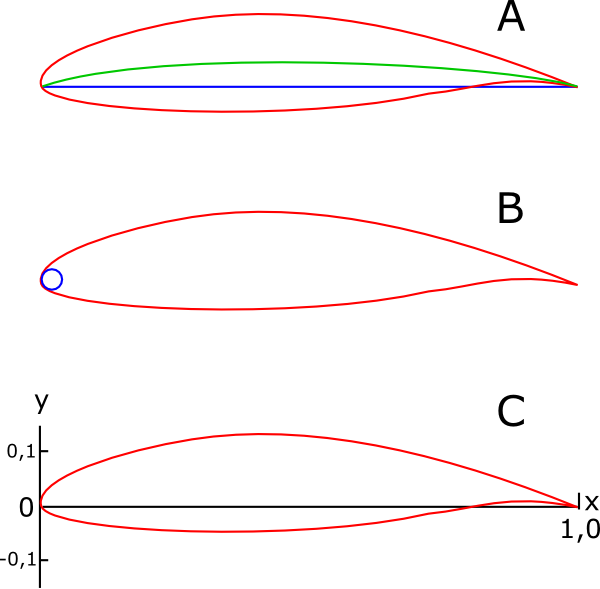
\includegraphics[scale=0.15]{images/airfoil.png}
\caption{NACA airfoil \cite{airfoil_wikipedia}}
\label{fig:nacaairfoil}
\end{figure}


\textit{ADD MORE AWESOME SCIENTIFIC PHYSICS STUFF HERE!!}

%################################################################################################################%

\section{Requirements}

The following sections pertain to the analysis of the functional and non-functional requirements of this specific software system.

\subsection{Functional Requirements}


\noindent\textbf{Start optimization execution:}
The web application in charge of managing the execution of the optimization procedures naturally allows for an authenticated user or administrator to start a brand new execution process. The administrator can also view previously recorded executions along with all their associated data.\\\par

\noindent\textbf{Setting up the optimization parameters:}
Before starting an execution, the user is presented with a series of inputs for the optimization parameters. These are used initially to start the optimization algorithm.\\\par

\noindent\textbf{Manage previous executions:}
The system also allows to view previously launched execution and study the gathered data in the form of text and graphs.\\\par


\noindent\textbf{Provide a log of important actions within the system:}
The user interface also provides a way of accessing all logged data from the system such as when a new account is created, when a connection from a user is registered, when optimization procedures are created, executed, deleted, etc.\\\par


\noindent\textbf{Optimize lift-to-drag ratio:}
The system should succeed in optimizing the lift to drag ratio carefully adjusting the parameters' values and study their effects on the lift and drag.\\\par

\noindent\textbf{Ability to plot the ratio over iterations:}
When an execution has finished successfully, and while the execution is taking place, a plot is continuously populated with the new data being calculated. The ratio between the lift and the drag is always updated after each iteration and the evolution of the value can be studied across all of the iterations.\\\par

\noindent\textbf{Ability to draw a sketch of the wing with the optimized parameters:}
Similarly to the previous requirement, a drawing of the wing with the optimized parameters is generated at each iteration and drawn to the screen for the user's consideration and study.\\\par






\subsection{Non-Functional Requirements}

\par
\textbf{Intuitive User Interface:}
One of the requirements of this system is that an intuitive user interface be built to be able to manage and control the underlying system and easily access log entries, optimization data and more. The user interface was built to be highly configurable and customizable allowing the user to easily navigate the interface through a series of self-explanatory icons for navigation which are always present on the left-hand side of the screen.\\\par

\noindent\textbf{System Resources:}
The system is meant to be optimized for a low consumption of system resources. In order to accommodate this requirement a lightweight Javascript framework was used that will save network bandwidth by only sending the required data through the wire. More of this is explained in section~\ref{subsec:Meteor} regarding to the Meteor framework.\\\par

\noindent\textbf{Security:}
Most systems nowadays require very strict and secure access in regards to authentication and permissions. Web applications are no exception, and as such, we included authentication using the secure shell protocol. More information can be found in section~\ref{sec:software_characteristics} \\\par

\noindent\textbf{Robustness:}
 The system should be able to continue the calculations after the application crashes on either client or server side. Our system recovers from errors like these by restarting from the last saved iteration with its corresponding parameters.\\\par

\noindent\textbf{Privacy:}
The system should allow each user to only have access to his/her previous computations. No optimizations should be shared by default\footnote{Sharing of optimizations between users will be made available in a future version.}.
 \\\par

\noindent\textbf{Open-source:}
The application should be open source as well as use open-source software.
\\\par

\noindent\textbf{Portability:}
The software should remain operable on various operating systems, browsers, and mobile devices.
\\\par


\noindent\textbf{Backup:}
The database should be backed up regularly.
\\\par





\subsection{Software System Characteristics}
\label{sec:software_characteristics}

\begin{itemize}
   \item  Reliability: A description of  how our system is reliable goes here...

   \item  \textit{Security:} We use SSH for authentication by connecting to the Astral cluster to make sure that the system is only used by a Cranfield team, but is developed in a way that makes it really easy to modify it for other authentication methods. SSH is a cryptographic network protocol that ensure that any data that goes through the wire in the authentication process is encrypted, by means of establishing a secure channel over the network which by definition is open to probing and attacks. The users passwords are stored in the database using a secure encryption method called Bcrypt, according to industry's best practices. 
   

   \item  \textit{Usability:} Even if a ``Help`` section is provided in the web application, we have considered the graphic interface as a highly important criteria to improve the user experience. 

   \item  \textit{Performance:} The client-server architecture of the web application implies that the computation is not operated by the user, thereafter the hardware of the user wouldn't be faulty in case of an excessive computation time. However, the elegance of the web interface depends on the user's software (web browser, operating system, Javascript version) or hardware (the computation power). Moreover, the frequency the web application is updated depends of the network throughput of the user. In this application, only the relevant parts of the website are updated, those which have changed by the time. This feature unloads both the server and client load.

   \item  \textit{Portability:} The system, due to having been built on top of a web stack makes it extremely portable. Any device with a connection to the Internet can access the interface and launch new optimizations right away, check logs for any required information and perform any relevant changes.

\end{itemize}

%################################################################################################################%

\section{Technology}

\subsection{Meteor}
\label{subsec:Meteor}

Meteor is a realtime web application framework which supports realtime interaction and reactivity out-of-the-box.

\subsubsection{Underlying Principles}

Meteor has some rather interesting characteristics that separate it from other platforms. It optimizes the quantity of data that needs to be sent to the client over the network. Since the client and the server execute the same exact code, Meteor doesn't send HTML through the wire, instead it sends the necessary data needed to render the page. It allows for the web application to be built using Javascript as the common programming language making it extremely lightweight and practically able to be executed in any browser that has Javascript enabled, which most do by default. On of the best strengths of this framework is the autonomy between the component it uses (called ``Smart Packages``), whatever they are official or supported by the Meteor community.\\\par

\noindent Another interesting characteristic of Meteor is that the database, where we store user information, optimization and log data, is accessible from both client and server. Moreover they are automatically synchronized, which means that any change that occurs in the database is automatically rendered in the client's view: the changes are pushed to the client. On these terms, Meteor introduces a concept called ``latency compensation``, which as its name indicates is a method to alleviate network latency. It consists in the emulation of a subset of the Mongo database from the server in the client itself. This way a copy of the necessary subset of data resides in the client and any changes are automatically propagated to the other Mongo instances. This prefetching of data makes it look like a call to the server is getting a response instantly.\\ 

\noindent In the following sections will be discussed how Meteor is tightly coupled with its embedded functionalities.

\subsubsection{Node.js}
The framework is built ontop of Node.js, and takes advantage of its concept and stability, however Meteor is not as mature as Node.js is and has several differences. Meteor uses the server of Node.js and the way it sends or receives the requests. Meteor doesn't use Node.js packaging system, but provides its own, even if it takes advantage of some Node.js packages.

\subsubsection{MongoDB}
The basic Meteor package incorporates a Mongo database, the only database it works with (for the time being). There is not setup required, as the Meteor environment is tied to its database. By working closely to a unique database, Meteor ensures in this way a close collaboration that leads to a tough synergy. Thus, the developers won't be concerned about the interaction between the database and the platform. As soon as the project is created, the database is initialised. They are only designing the tables, and calling the requests.\\\par
\noindent MongoDB is a cross-platform document-oriented database based on a NOSQL concept. It's not a SQL database since it has its own concepts. Consequently, instead of breaking down a functional concept into relational structures, the functional concept is stored into a small number of complete documents. For instance, where a SQL approach would break down the concept of a car into several pieces (engine, wheels) and separate the manufacturer into another table, the document-oriented approach will rather have a complete "object" for the car embedding the manufacturer information and the difference pieces of the car. In this way, the functional concept is comprehended intuitively and naturally, which makes it easier to work with.

\subsubsection{Login Package}
Meteor already implements a log in service, as it's a redundant requirement on web designing, although the developers have the eventuality to write their own package. The community also makes available several packages maintained by the Meteor Project, such as third-party authentication services (Google Accounts, Facebook Accounts, and so on).\\\par


\subsubsection{CoffeeScript}
In order to make easier the code writing, as well for the client side as the server side, we have chosen to use a package as a verbose overlay of the Javascript language: CoffeeScript. Coffeescript compiles one-to-one into the Javascript instructions, whereas it improves the readability and the brevity of the language (which corresponds to the concept of a syntactic sugar), and moreover add some useful features. In this way, using CoffeeScript doesn't slow down the execution.

\subsubsection{Free Hosting service}
For every project developed, a basic free hosting space, hosted on a sub-domain of Meteor or another domain. This hosting service is as interesting as Meteor is meant to develop some quick prototypes or web applications, and not complex ones.


%################################################################################################################%


\section{System Design}

The design of the system is key to any software project because it studies the way that the software will meet the requirements mentioned above.

- Class diagram
- Use case diagrams

%################################################################################################################%


\section{Implementation of System}

\section{System test and validation}

\section{Failure case studies}

\section{Conclusion}

\section{Appendix}



%################################################################################################################%


\subsection{System installation}

A list of instructions on the installation procedure can be found on the official code repository on Github that can be found at \url{https://github.com/mathieudutour/group-project}. For reference, we will describe the process step-by-step with screenshots to aid the user. As a sidenote the system has already been deployed to the Meteor domain under the \emph{http://group-project.meteor.com/} subdomain, so if needed, no further installation is required to test the application. The first step is to install the Meteor framework. This can be easily carried out through the command line with the following command:

\vspace{5mm} %5mm vertical space

\begin{lstlisting}[language=sh]
curl https://install.meteor.com/ | sh
\end{lstlisting}

\vspace{5mm} %5mm vertical space

\noindent This will install the meteor executable file in our system and will make sure that it is usable from anywhere in our system. If you are not able to install Meteor because you are running Windows or for any other reason, we recommend you to use Nitrous.io.\\

\noindent\textbf{Nitrous.io} is an online service that allows you to edit and write code directly on the cloud from  your browser as well as run applications from within the service. You can find a blog post on how to configure the service to develop Meteor applications \textit{\href{https://www.discovermeteor.com/blog/meteor-nitrous}{here}}.\\

\noindent The next step is to download the source code for the project. This can be done by using Git, a popular version control system, using the following command:

\vspace{5mm} %5mm vertical space


\begin{verbatim}
$ git clone https://github.com/mathieudutour/group-project
\end{verbatim}


\vspace{5mm} %5mm vertical space

\noindent Once the project has been cloned into your current directory you are almost ready to run it. The project consists of several different packages that need to be correctly referenced in order for the program to execute successfully. This is done by creating a symlink to the packages.

\vspace{5mm} %5mm vertical space

\begin{verbatim}
cd group-project/
ln -s /absolute/path/to/group-project:authentication 
monitor/packages/group-project:authentication
\end{verbatim}




\vspace{5mm} %5mm vertical space

\noindent Please note that the \textit{ln} command has been broken into two lines to fit the page. There should only be a single a space between the directories. This command must be executed for all the packages in the project. These are outlined below:

\begin{itemize}
  \item group-project:authentication
  \item group-project:drag-solver
  \item group-project:lift-solver
  \item group-project:optimizer
\end{itemize}

It is also of relevant importance to make sure that the absolute path is set to your specific directory where the project has been cloned to. After this has been completed for all the packages we can proceed to run the project with meteor. This is done by entering the `monitor' directory and typing ``meteor'' to run the application.

\vspace{5mm} %5mm vertical space

\begin{lstlisting}[language=sh]
cd monitor/
meteor
\end{lstlisting}

\vspace{5mm} %5mm vertical space

\begin{figure}[h!]
  \centering
    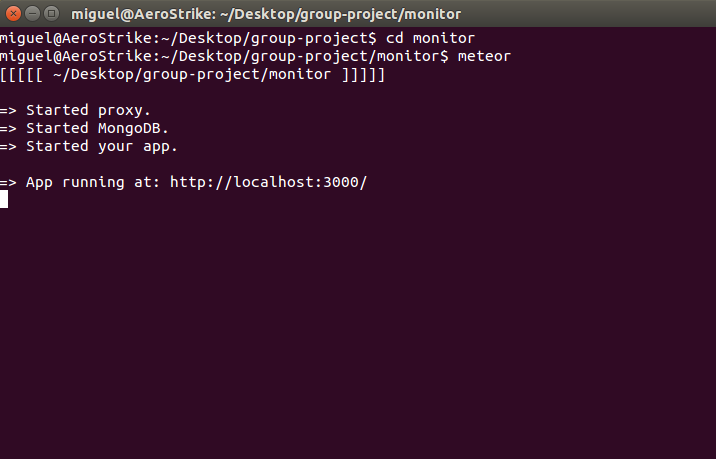
\includegraphics[scale=0.6]{images/app_running.png}
  \caption{Starting the application.}
\end{figure}


\vspace{2mm} %5mm vertical space

After Meteor has finished starting the database, loading packages, plugins, and building the application, a message will appear stating that the application is running at a certain address. Usually this will be localhost and port 3000 by default. 



%################################################################################################################%

\subsection{System operation manual}

Now that we have the application installed and running on our local server we can proceed to understand how the application works and is operated. At first sight, as we can see in Figure~\ref{fig:AppMain}, we can see the different options available on the left sidebar of the main screen. These include:

\begin{itemize}
  \item Optimizations
  \item Logs
  \item Settings
  \item Help
  \item About
\end{itemize}

\begin{figure}[h!]
  \centering
    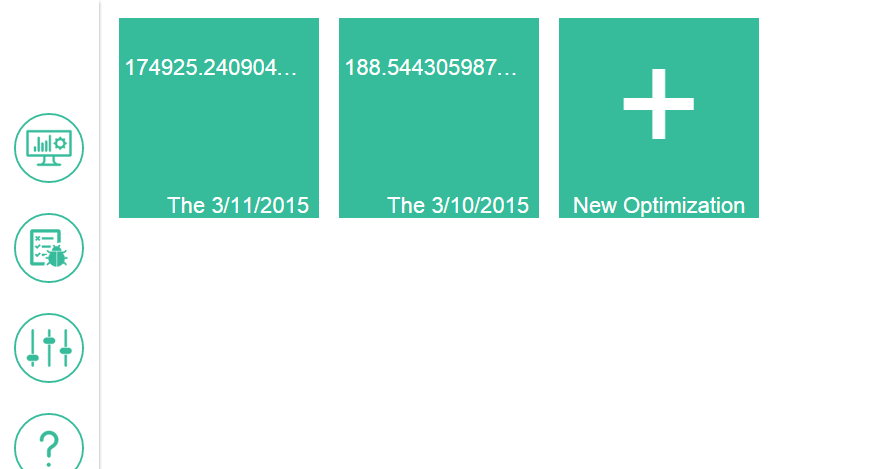
\includegraphics[scale=0.35]{images/optimizations.png}
  \caption{The main screen of application when it is first launched.}
  \label{fig:AppMain}
\end{figure}

Through the ``Optimizations'' option, as seen again in Figure~\ref{fig:AppMain}, we can view other previously executed optimizations as well as an option to create a new optimization execution. By clicking on the "New Optimization" button we are presented with a form to fill in some initial values for some of the parameters to be optimized. When we are happy with the initial values that will be fed into the optimizer we can click on `Go!' which will automatically load the results page and execute a single iteration as seen in Figure~\ref{fig:OptimizationResults}. We can observe how the drawing of the wing is generated for the single iteration of the optimizer. To perform more iterations we can simply click on the `Iterate' button to iterate the default number of times that is configured in the Settings menu.

\begin{figure}[h!]
  \centering
    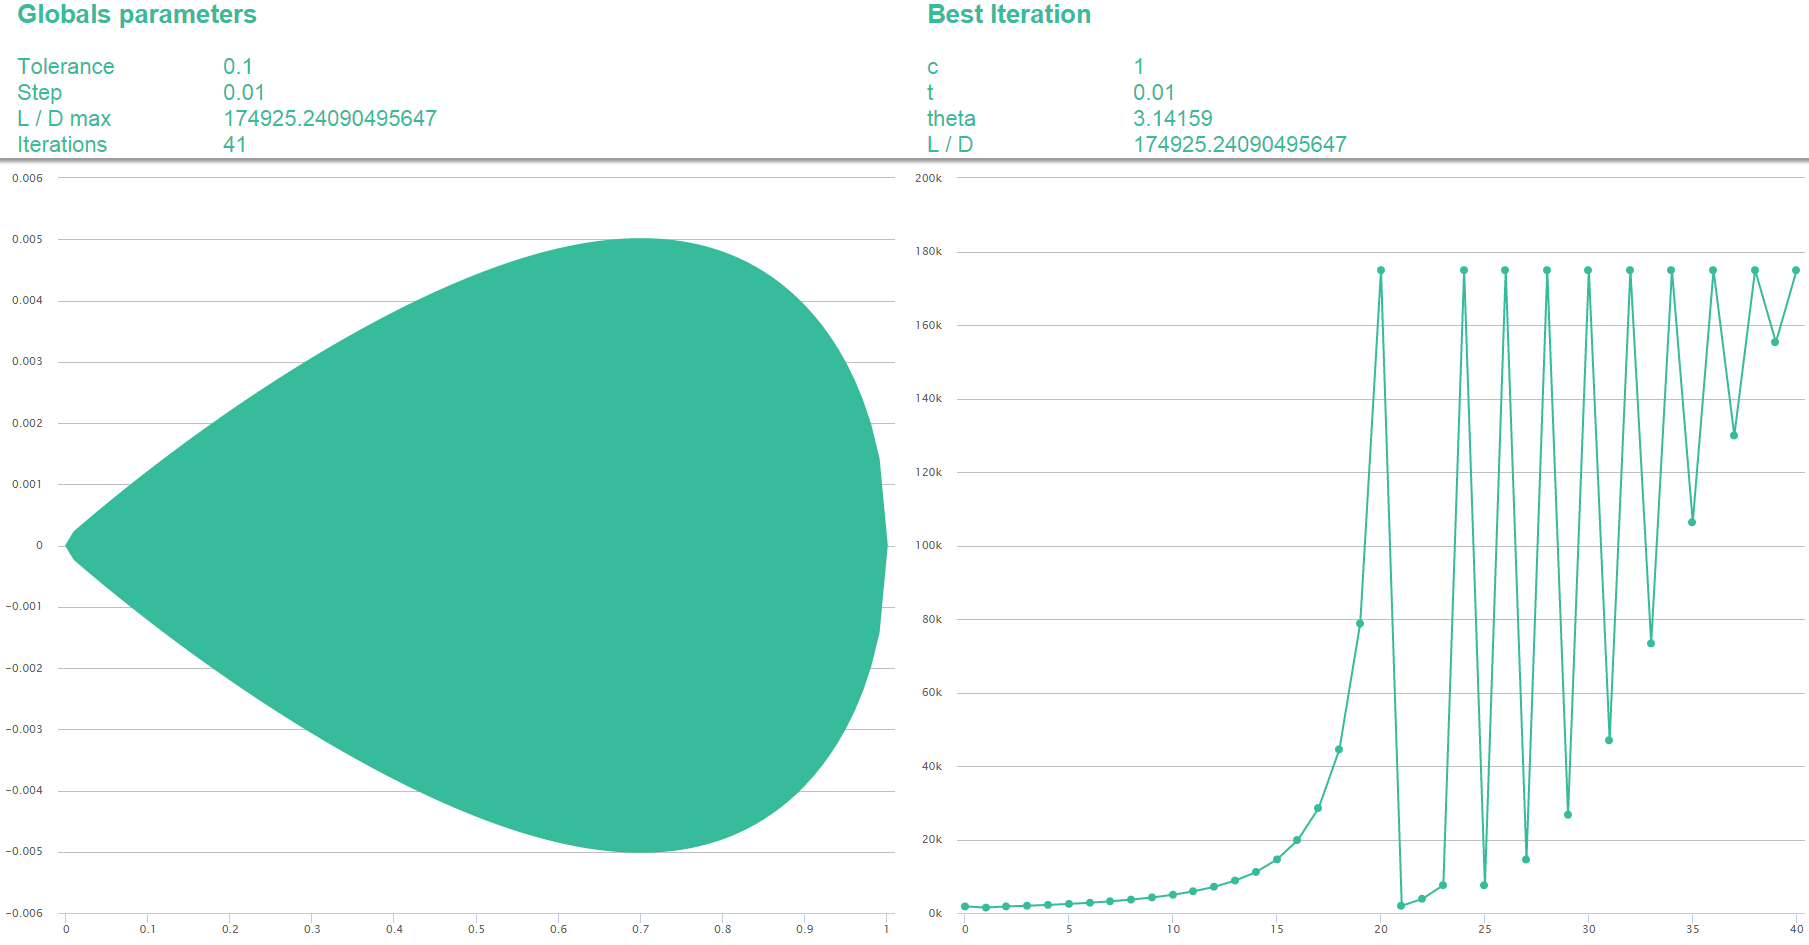
\includegraphics[scale=0.20]{images/optimizations_res.png}
  \caption{Results of an optimization process.}
  \label{fig:OptimizationResults}
\end{figure}

The next section is the ``Log'' section, where a log is kept of all user interaction, such as account creation, user login, creation of optimizations, performing iterations, and lastly finishing an optimization process. These logs are persistent by means of the Mongo database and are therefore accessible at all times by any user with credentials to the system. Any unauthorized user will have no access to this, or any other data.


The ``Settings'' section (Figure~\ref{fig:settings_image}) allows the user to quickly wipe all optimizations from the system in order to facilitate and quicken the time needed to perform this task in case the optimization count gets too high to do manually. The user is also allowed to change the overall color theme between the default `Emerald Green' theme, `Sapphire Blue', and `Ruby Red'. Another important setting that is adjustable from the settings is the number of iterations that the optimizer should perform every time the button `Iterate' is clicked. The user can set this to view the data after a certain desired number of iterations. Lastly, to clear the session, a log out button is provided to exit the application. 

\begin{figure}[h!]
  \centering
    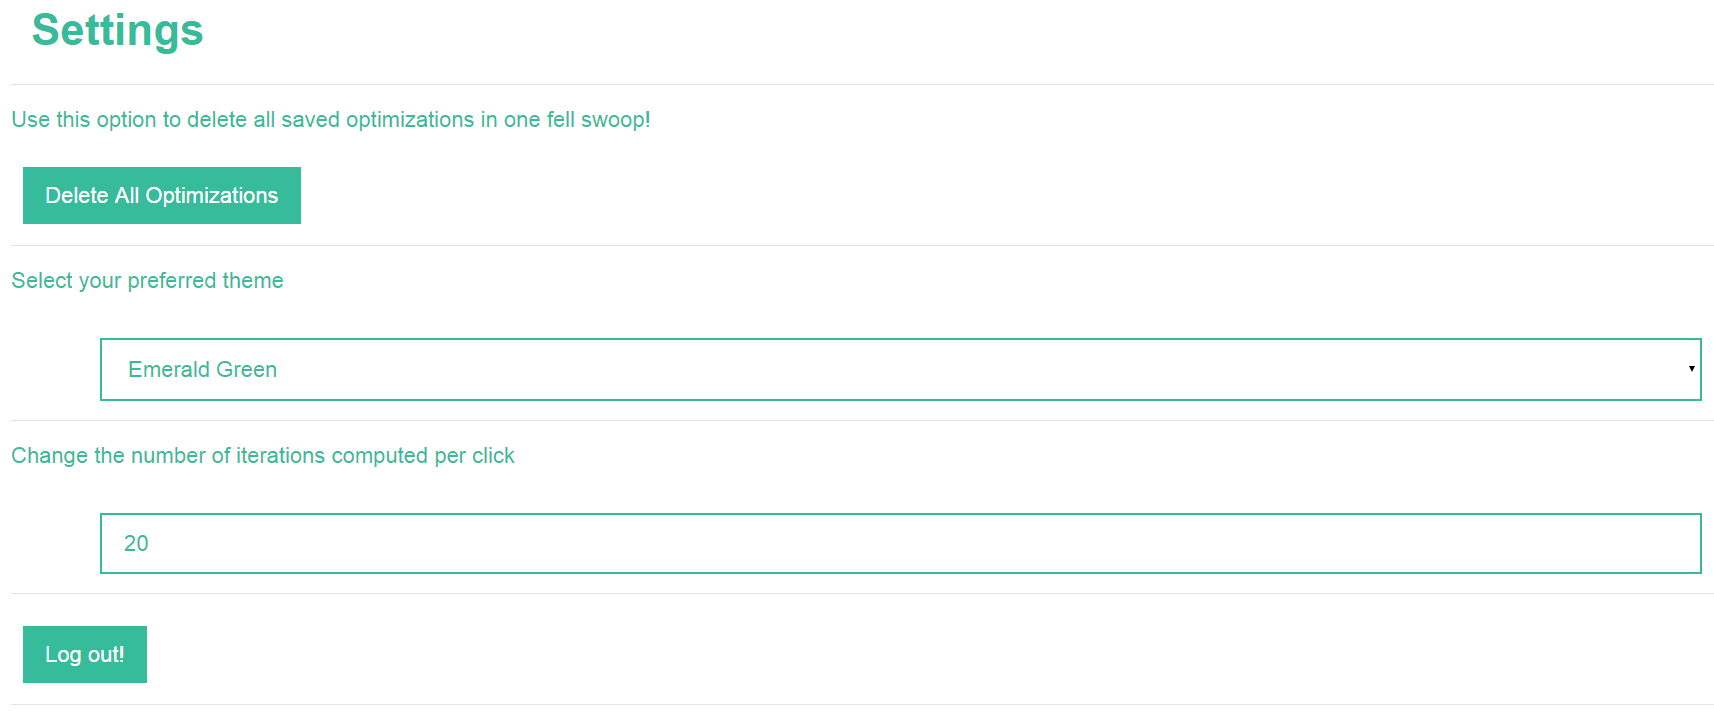
\includegraphics[scale=0.3]{images/settings.png}
  \caption{Different options in the settings menu.}
  \label{fig:settings_image}
\end{figure}

The ``Help'' section and ``About'' sections are self-explanatory. The former aims to explain how to use the optimizer by explaining the optimization creation process step-by-step. The latter shows the name and image of the developers.


%################################################################################################################%



\bibliographystyle{unsrt}
\bibliography{references}

\end{document}
